\documentclass{article}

% Formatting
\usepackage[utf8]{inputenc}
\usepackage[margin=1in]{geometry}
\usepackage[titletoc,title]{appendix}
\usepackage{polski}
\usepackage[polish]{babel}


\usepackage{graphicx,float}
\graphicspath{ {./images/} }


% Title content
\title{Przykłady modelowania i analizy systemów
współbieżnych z wykorzystaniem sieci Petri.}
\author{Jakub Myśliwiec}
\date{07 Styczeń 2020}

\begin{document}

\maketitle


\section{Symulacja i analiza własnego przykładu}

\subsection{Symulacja}
\subsection{Graf osiągalności}
\subsection{Analiza niezmienników przejść}

\section{Symulacja sieci z rysunku}
\begin{figure}[H]
    \centering
    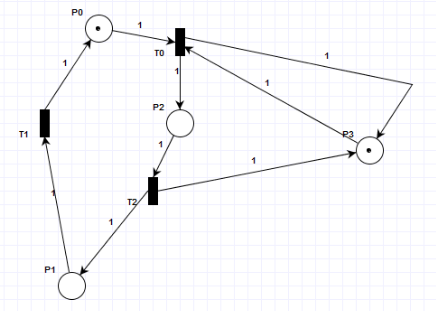
\includegraphics[width=0.8\textwidth, height=0.4\textheight]{zad2.png}
    \caption{Sieć do analizy}
\end{figure}

\subsection{Analiza niezmienników przejść}
\begin{figure}[H]
    \centering
    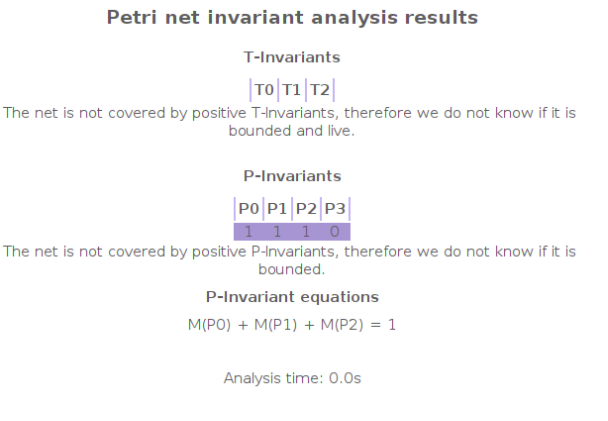
\includegraphics[width=0.8\textwidth, height=0.4\textheight]{zad2_analiza.png}
    \caption{Analiza sieci}
\end{figure}

Odwracalność cechuje się możliwością wrócenia do stanu początkowego. 
W analizie niezmienników zauważmy, że nie ma żadnych niezmienników tranzycji (T-invariants).
Wynika z tego że nie możemy odpalić tranzycji w taki sposób by wrócić do markowania początkowego,
czyli sieć nie jest odwracalna. 

\subsection{Graf osiągalności}
\begin{figure}[H]
    \centering
    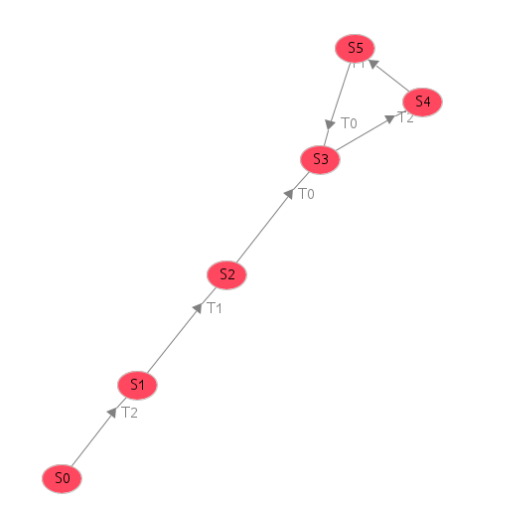
\includegraphics[width=0.8\textwidth, height=0.4\textheight]{zad2_graph.png}
    \caption{Graf osiągalności}
\end{figure}

Sieć jest żywa, gdyż począwszy od stanu początkowego zostanie uruchomione każde przejsćie.
Nie występuje żadne martwe przejście.Sieć nie jest ograniczona gdyż miejsce \textbf{P3}
nie jest ograniczone. Jak widać w grafie sieć wpada w nieskończony cykl między stanami \textbf{S3, S4, S5}
i liczba tokenów w \textbf{P3} będzie rosła w nieskończoność.

\section{Wzajemne wykluczanie dwóch procesów na wspólnym zasobie}
\begin{figure}[H]
    \centering
    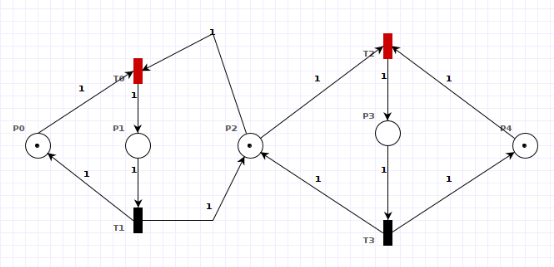
\includegraphics[width=0.8\textwidth, height=0.4\textheight]{zad3.png}
    \caption{Sieć wykluczających się procesów dla wspólnego zasobu}
\end{figure}

\subsection{Symulacja}
\begin{figure}[H]
    \centering
    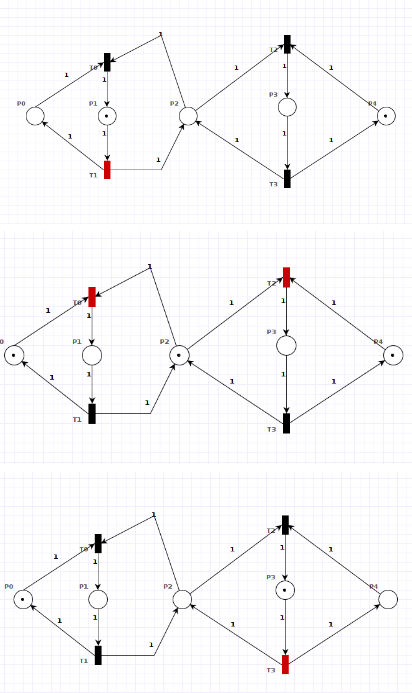
\includegraphics[width=0.8\textwidth, height=0.9\textheight]{zad3_simulation.png}
    \caption{Symulacja działania sieci}
\end{figure}

Jak widać procesy wzajemnie wykluczają dostęp do zasobu i raz w sekcji krytycznej znajduję
się proces po lewej stronie a raz po prawej.

\subsection{Analiza niezmienników}
\begin{figure}[H]
    \centering
    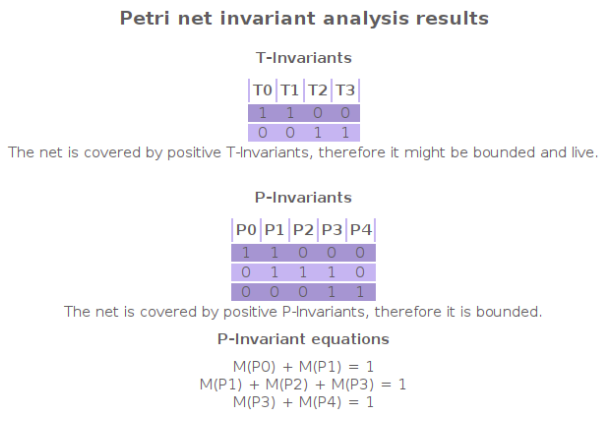
\includegraphics[width=0.8\textwidth, height=0.4\textheight]{zad3_analiza.png}
    \caption{Analiza sieci}
\end{figure}

Równanie \textbf{M(P0) + M(P1) = 1} świadczy o tym, że proces po lewej stronie
nie możę być 2 dwóch stanach równocześnie, albo będzie 
posiadał zasób albo nie. \\
Analogiczna sytuacja zachodzi dla drugiego procesu (po prawej stronie)
\textbf{M(P3) + M(P4) = 1}.

Równaniem ukazującym działanie sekcji krytycznej jest 
\textbf{M(P1) + M(P2) + M(P3) = 1}. 
Pokazuje to, że w danym momencie tylko jedno z miejsc 
może posiadać token więc 2 procesy nie znajdą się w tym samym momencie w sekcji krytycznej. 

\section{Problem konsumenta i producenta}
\begin{figure}[H]
    \centering
    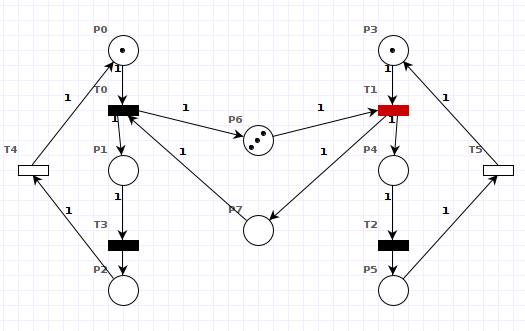
\includegraphics[width=0.8\textwidth, height=0.4\textheight]{zad4.png}
    \caption{Sieć dla problemu producenta i konsumenta}
\end{figure}

\subsection{Analiza niezmienników}
\begin{figure}[H]
    \centering
    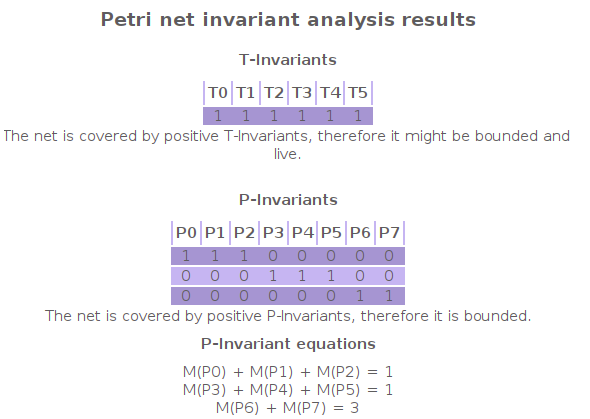
\includegraphics[width=0.8\textwidth, height=0.4\textheight]{zad4_analiza.png}
    \caption{Analiza sieci}
\end{figure}

Sieć jest zachowawcza gdyż liczba tokenów w sieci 
jest stała, nie zmienia się. Zawsze są 3 tokeny w buforze i po jednym
w procesie producenta i konsumenta.
O rozmiarze bufora świadczy ostatnie równanie
\textbf{M(P6) + M(P7) = 3} i wynosi on \textbf{3}.

\section{Problem producentów i konsumentów z nieskończonym buforem}
\begin{figure}[H]
    \centering
    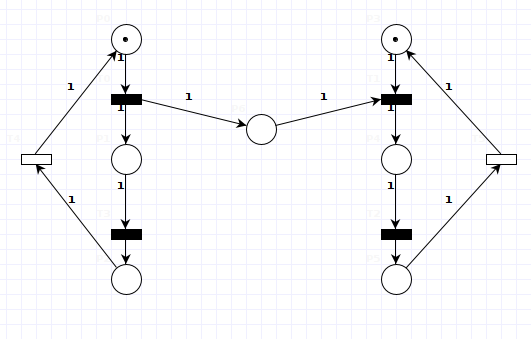
\includegraphics[width=0.8\textwidth, height=0.4\textheight]{zad5.png}
    \caption{Sieć dla problemu z nieskończonym buforem}
\end{figure}

\subsection{Analiza niezmienników}
\begin{figure}[H]
    \centering
    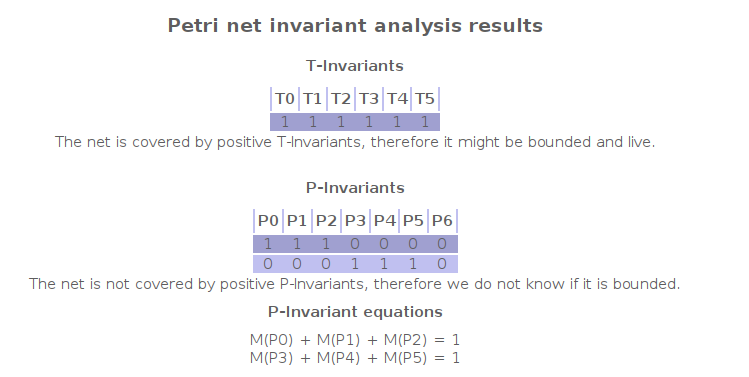
\includegraphics[width=0.8\textwidth, height=0.4\textheight]{zad5_analiza.png}
    \caption{Analiza sieci}
\end{figure}

Jak widać z analizy niezmienników zawsze w procesach producenta i konsumenta będzię po jednym tokenie.
Natomiast w buforze \textbf{P6} nie ma takiego ograniczenia (0 w wektorach P-Invariants), czyli mogą się tam gromadzić tokeny w
nieskończoność, co oznacza że poprawnie skonstruowałem sieć z buforem nieograniczonym.

\section{Problem zastoju meksykańskiego}
\begin{figure}[H]
    \centering
    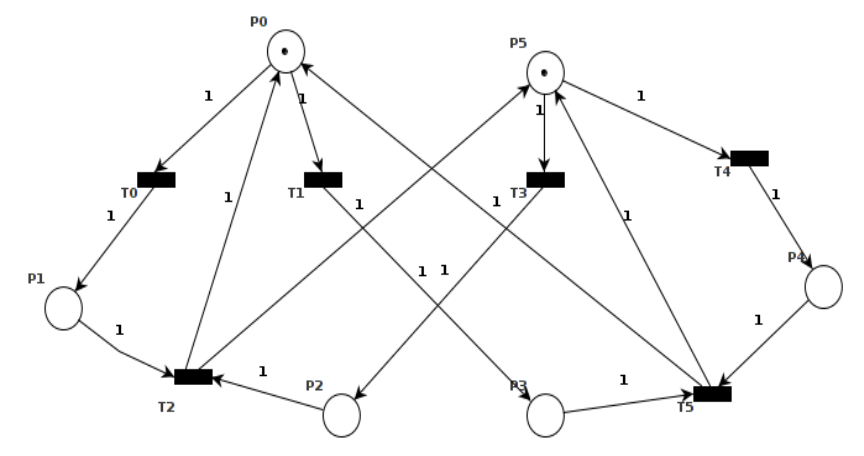
\includegraphics[width=0.8\textwidth, height=0.4\textheight]{zad6.png}
    \caption{Sieć dla problemu z zastoju meksykańskiego}
\end{figure}

\subsection{Graf osiągalności}
\subsection{State Space Analysis}

\section{Zakleszczenie}
\begin{figure}[H]
    \centering
    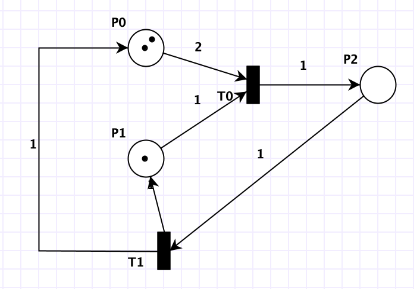
\includegraphics[width=0.8\textwidth, height=0.4\textheight]{zad7.png}
    \caption{Mój projekt sieci prezentujący zakleszczenie}
\end{figure}

\subsection{Graf osiągalności}
\begin{figure}[H]
    \centering
    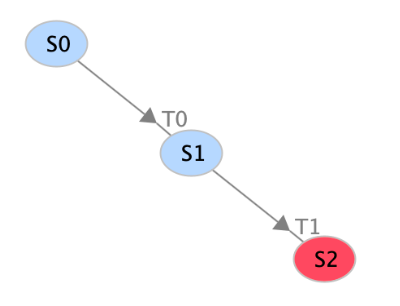
\includegraphics[width=0.8\textwidth, height=0.4\textheight]{zad7_graph.png}
    \caption{Graf osiągalności}
\end{figure}

Jak widzimy sieć zakleszcza się po przejściu \textbf{T1}.
Wynika to z tego, że tranzycja \textbf{T0} wymaga pobrania 2 tokenów od miejsca 
\textbf{P0} oraz jednego tokenu od \textbf{P1}, natomiast do obu miejsc po 
tranzycji \textbf{T1} dotrze po jednym tokenie.

\subsection{State space analysis}
\begin{figure}[H]
    \centering
    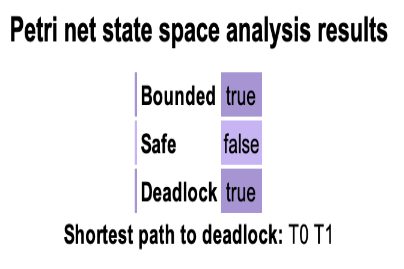
\includegraphics[width=0.8\textwidth, height=0.4\textheight]{zad7_analiza.png}
    \caption{Analiza stanów}
\end{figure}

Jak widzimy \textit{State space analysis} wykazało, że w sieci jest zakleszczenie.

\section{Problem 5 filozofów}
\begin{figure}[H]
    \centering
    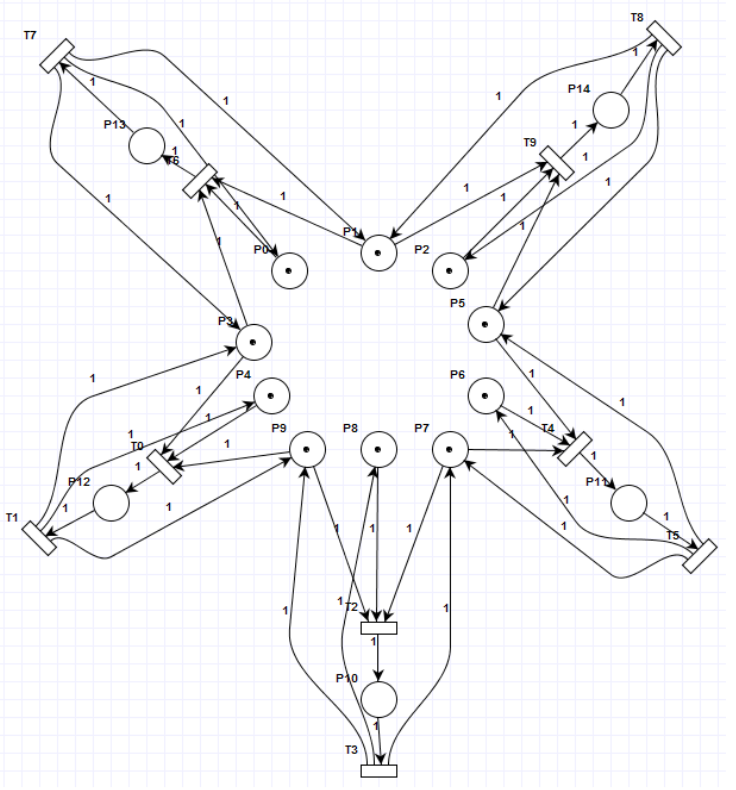
\includegraphics[width=0.8\textwidth, height=0.7\textheight]{zad8.png}
    \caption{Sieć dla problemu 5 filozofów}
\end{figure}

\end{document}